\documentclass[a4paper,11pt,reqno]{amsart}
\usepackage{M4ParcRenf}
\usepackage{tikz,tkz-tab}

% \solutionstrue

\begin{document}

% ==================================
\hautdepage{

\ifsolutions{Solutions de l'interrogation}\else{Interrogation}\fi\par\normalfont\normalsize
28 mars 2018\\{[ durée: 1 heure ]}\par
}
% ==================================
\ifsolutions\else
% {\fontencoding{U}\fontfamily{futs}\selectfont\char 66\relax}
\tikz[baseline=(e.base)]{\NoAutoSpacing\node(e){!};\draw[red,ultra thick,line join=round,yshift=-.15ex](90:1em)--(210:1em)--(330:1em)--cycle;}
\textbf{Les documents et les calculatrices ne sont pas autorisés.}

\hfill
\fi

%-----------------------------------
\begin{exo}

  On considère pour $n\in\mathbb{N}$ la fonction $f_{n}=\frac{nx}{1+(nx)^3}$.
  \begin{enumerate}
    \item Étudier la convergence simple et uniforme de la suite $(f_{n})_{n\geq 1}$ sur $\mathbb{R}_{+}$ et sur $[\varepsilon,\infty[$ pour $\varepsilon>0$.

    \item Étudier la convergence simple et uniforme de la série $\sum_{n\geq 1}f_{n}$ sur ces mêmes ensembles.
  \end{enumerate}
\end{exo}

\begin{solution}
  \begin{enumerate}
    \item Soit $f(x)=\frac{x}{1+x^3}$. Nous avons $f'(x)=\frac{(1+x^3)-x(3x^2)}{(1+x^3)^2} = \frac{1-2x^3}{(1+x^3)^2}$, d'où la tableau de variations
    \begin{center}\scalebox{.77}{
      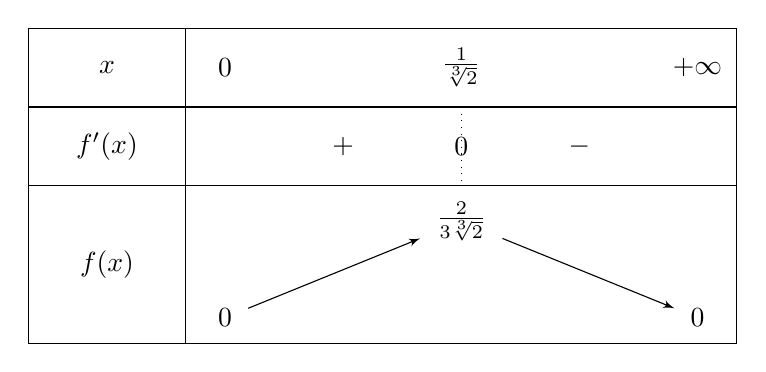
\begin{tikzpicture}
        \tkzTabInit{$x$ / 1 , $f'(x)$ / 1, $f(x)$ / 2}{$0$, $\frac{1}{\sqrt[3]{2}}$, $+\infty$}
        \tkzTabLine{,+,z, -}
        \tkzTabVar{-/ 0, +/ $\frac{2}{3\sqrt[3]{2}}$, -/ 0}
      \end{tikzpicture}
    }
    \end{center}
    et donc $\sup_{\mathbb{R}_{+}}|f|=f(\frac{1}{\sqrt[3]{2}}) > 0$. De plus $\lim_{x\to\infty}f(x)=0$.\\
    Comme $f_{n}(x)=f(nx)$, nous avons d'après l'étude de $f$ que pour $x>0$, $\lim_{n\to\infty}f_n(x)=\lim_{n\to\infty}f(nx)=0$ et comme $f_{n}(0)=0$, on trouve la limite simple $\lim_{n\to\infty}f_n=0$ sur $\mathbb{R}_{+}$. Par contre comme $\sup_{\mathbb{R}_{+}}|f_n|=\sup_{\mathbb{R}_{+}}|f|\nrightarrow 0$, la suite $(f_{n})_{n\geq 1}$ ne converge pas uniformément sur $\mathbb{R}_{+}$.\\
    Soit $\varepsilon>0$, pour $n$ assez grand ($n>\frac{1}{\varepsilon}(\frac{1}{\sqrt[3]{2}})$), la fonction $f_{n}$ est positive et décroissante sur $[\varepsilon,\infty[$, donc $\sup_{[\varepsilon,\infty[}|f_n|=f_{n}(\varepsilon) = f(n\varepsilon) \to 0$ quand $n\to 0$. Ainsi la suite $(f_{n})_{n\geq 1}$ est uniformément convergente sur $[\varepsilon,\infty[$ pour $\varepsilon>0$.

    \item Pour $x=0$, $\sum_{n\geq 1}f_{n}(0)=0$. Pour $x>0$, $f_{n}=\frac{nx}{1+(nx)^3}\sim\frac{1}{(nx)^2}$ quand $n\to\infty$, et donc $\sum_{n\geq 1}f_{n}$ converge car $\sum_{n\geq 1}\frac{1}{(nx)^2} = \frac{1}{x^2}\sum_{n\geq 1}\frac{1}{n^2}$ converge. Ainsi $\sum_{n\geq 1}f_{n}$ converge simplement sur $\mathbb{R}_{+}$. Mais d'après la question précédente, cette convergence n'est pas uniforme, car la suite $(f_{n})_{n\geq 1}$ ne converge pas uniformément (vers $0$) sur $\mathbb{R}_{+}$.\\
    De même que dans la question précédente, pour $n$ assez grand $\sup_{[\varepsilon,\infty[}|f_n|=f_{n}(\varepsilon)$ et comme la série $\sum_{n\geq 1}f_{n}(\varepsilon)$ converge (d'après la convergence simple), alors $\sum_{n\geq 1}f_{n}$ converge normalement, et donc uniformément, sur $[\varepsilon,\infty[$.
  \end{enumerate}
\end{solution}

%-----------------------------------
\begin{exo}

  \emph{L'équation $y''(x)=-y(x)$, sur tout intervalle de $\mathbb{R}$ contenant $0$, admet une unique solution qui vérifie les conditions initiales $y(0)=0$ et $y'(0)=1$, cette solution est appelée $\sin(x)$. Il existe également une unique solution qui vérifie les conditions initiales $y(0)=1$ et $y'(0)=0$, cette solution est appelée $\cos(x)$.
  On rappelle que la fonction exponentielle est la valeur de la série $e^{z} = \sum_{k=0}^{\infty}\frac{z^{k}}{k!}$ pour $\forall z \in \mathbb{C}$.}

  \begin{enumerate}
    \item Montrer que $\sin(x)=\sum_{k=0}^{\infty}\frac{(-1)^{k}x^{(2k+1)}}{(2k+1)!}$ et $\cos(x)=\sum_{k=0}^{\infty}\frac{(-1)^{k}x^{(2k)}}{(2k)!}$ pour $\forall x \in \mathbb{R}$.
    \item Montrer la formule d'Euler $e^{ix}=\cos(x) + i\sin(x)$ pour $x\in \mathbb{R}$.
  \end{enumerate}
\end{exo}

\begin{solution}

\begin{enumerate}
  \item Soient $e_{k}(x) = \frac{x^{k}}{k!}$, $c_{k}(x)=\frac{(-1)^{k}x^{(2k)}}{(2k)!} = (-1)^{k}e_{2k}(x)$ et $s_{k}(x)=\frac{(-1)^{k}x^{(2k+1)}}{(2k+1)!} = (-1)^{k}e_{2k+1}(x)$. Sur l'intervalle $[-M,M]$ nous avons $\sup_{[-M,M]}e_{n} = e_{n}(M)$ et comme la série $\sum e_{n}(M)$ converge (et a pour valeur $e^{M}$), on peut conclure que les séries $\sum_{k=0}^{\infty}(-1)^{k}e_{2k}$ et $\sum_{k=0}^{\infty}(-1)^{k}e_{2k+1}$ convergent normalement, et donc uniformément, sur cet intervalle. De même, comme $e_k'=e_{k-1}$ pour $k\geq1$ et $e_0'=0$, les séries dérivées $\sum_{k=1}^{\infty}(-1)^{k}e_{2k-1}$ et $\sum_{k=0}^{\infty}(-1)^{k}e_{2k}$, ainsi que les séries dérivées secondes $\sum_{k=1}^{\infty}(-1)^{k}e_{2k-2}$ et $\sum_{k=1}^{\infty}(-1)^{k}e_{2k-2}$ convergent normalement sur $[-M,M]$.\\
  D'après ces convergences uniformes nous pouvons intervertir la somme et la dérivée et en utilisant $s_{k}'=c_{k}$, $c_{k}'=-s_{k-1}$ et $c_{0}'=0$ on obtient
  \begin{gather*}
    \left( \sum_{k=0}^{\infty}s_{k}(x) \right)'' = \sum_{k=1}^{\infty}-s_{k-1}(x) = -\sum_{k=0}^{\infty}s_{k}(x)\text{,}\\
    \left( \sum_{k=0}^{\infty}s_{k}(x) \right)_{x=0} = \sum_{k=0}^{\infty}s_{k}(0)=0\quad\text{et}\quad
    \left( \sum_{k=0}^{\infty}s_{k}(x) \right)_{x=0}' = \sum_{k=0}^{\infty}c_{k}(0)= 1\text{,}
  \end{gather*}
  et donc $\sin(x)=\sum_{k=0}^{\infty}s_{k}(x)$ sur $[-M,M]$ pour $\forall M > 0$. Par conséquent ces deux fonctions coïncident sur tout le $\mathbb{R}$. De même
  \begin{gather*}
    \left( \sum_{k=0}^{\infty}c_{k}(x) \right)'' = \sum_{k=1}^{\infty}-c_{k-1}(x) = -\sum_{k=0}^{\infty}c_{k}(x)\text{,}\\
    \left( \sum_{k=0}^{\infty}c_{k}(x) \right)_{x=0} = \sum_{k=0}^{\infty}c_k(0)= 1\quad\text{et}\quad
    \left( \sum_{k=0}^{\infty}c_{k}(x) \right)_{x=0}' = \sum_{k=1}^{\infty}-s_{k-1}(0)=0\text{,}
  \end{gather*}
  et donc $\cos(x)=\sum_{k=0}^{\infty}c_{k}(x)$ sur $[-M,M]$ pour $\forall M > 0$. Par conséquent ces deux fonctions coïncident sur tout le $\mathbb{R}$.
  \item En remplaçant $x$ par $ix$ dans la série entière de l'exponentielle et en utilisant les expressions en séries entières de $\sin(x)$ et de $\cos(x)$ démontrées dans la question précédente, on trouve
  $$
    e^{ix} = \sum_{k=0}^{\infty}\frac{(ix)^{k}}{k!} = \underbrace{\sum_{k=0}^{\infty}\frac{(-1)^k x^{(2k)}}{(2k)!}}_{\text{Les termes pairs}} + \underbrace{\sum_{k=0}^{\infty}\frac{i(-1)^k x^{(2k+1)}}{(2k+1)!}}_{\text{Les termes impairs}} = \cos(x) + i\sin(x).
  $$
\end{enumerate}

\end{solution}


\end{document}


